\section{英語表現2(谷野)}
\noindent \textbf{1.  以下の英文が完成するように(\quad)内に適切な関係詞を書きなさい．}{\scriptsize(2$\times$5)}\par
(1) This is the computer (\quad\quad) Mr.Tanino uses for his research.\par\quad
  (これは谷野先生が研究に使っているパソコンです)\par
(2) You can use (\quad\quad) topic is related to Osaka or technology.\par\quad
  (大阪かテクノロジーに関連したトピックであれば，どちらでも構いません)\par
(3) You can add (\quad\quad) toppings you like to your coffee.\par\quad
  (コーヒーにはお好きなトッピングを追加できます)\par
(4) I know a shop (\quad\quad) you can eat the best ramen in Osaka.\par\quad
  (大阪で一番美味しいラーメンが食べられるお店を知っています)\par
(5) (\quad\quad) surprised me was the strong flavor of the coffee.\par\quad 
  (私を驚かせたのは，コーヒーの強い風味でした)\par
\bigskip

\noindent \textbf{2.  以下の英文が完成するように(\quad)内に適切な語句(関係詞だけとは限りません)を書きなさい．}{\scriptsize(2$\times$10)}\par
(1) I met a woman (\quad\quad) spoke French well.\par
(2) This is the book (\quad\quad) he wrote.\par
(3) This house (\quad\quad) roof is red is my uncle's.\par
(4) This is the CD (\quad\quad)(\quad\quad) I told you.\par
(5) The hotel (\quad\quad) we stayed was wonderful.\par
(6) I remember the day (\quad\quad) I first met you.\par
(7) Tell me (\quad\quad)(\quad\quad) why you were late.\par
(8) That's (\quad\quad) the accident happened.\par
(9) I don't hear (\quad\quad) she said.\par
(10) I give you (\quad\quad) you want.\par
\bigskip\bigskip

\noindent \textbf{3.  以下の(\quad)内の語を与えられた日本語を参考にして並べ替え，(\quad)内で左から\underbar{2番目と4番目}に入る語を，記}\par\textbf{号で答えなさい．文頭の文字も小文字にしています．}{\scriptsize(2$\times$5)}\par
(1) (ア. happy イ. is ウ. makes エ. Mr. Tanino オ. what) ramen.\par\quad
  谷野先生を幸せにするものはラーメンです．\par
(2) Mr. Tanino (ア. amazing イ. brews ウ. coffee エ. smells オ. which) in the morning.\par\quad
  谷野先生は朝には素晴らしい香りのコーヒーを淹れ(brew)ます．\par
(3) Mr. Tanino has (ア. a イ. for beer ウ. friend エ. inspired オ. love カ. whose) him.\par\quad
  谷野先生には，そのビール愛が彼に影響を与えた友人がいます．\par
(4) Mr. Tanino works (ア. a イ. brewer ウ. he エ. met オ. overseas カ. whom キ. with).\par\quad
  谷野先生は海外で知り合った醸造家(brewer)と働いている．\par
(5) (ア. a イ. cup ウ. is エ. offered オ. Mr. Tanino カ. visits キ. whoever) of coffee.\par\quad
  谷野先生を訪ねる人はだれでもコーヒーが提供されます．\par
\bigskip\bigskip

\noindent \textbf{4.  以下の(\quad)内の語を文法的に正しく並べ替え，(\quad)内で左から\underbar{2番目と4番目}に入る語を，記号で答えなさい．}\par\textbf{文頭の文字も小文字にしています．}{\scriptsize(2$\times$10)}\par
(1) That woman is a (ア. are イ. books ウ. selling エ. whose オ. writer) well.\par
(2) This is a (ア. built イ. house ウ. twenty years エ. was オ. which) ago.\par
(3) The (ア. are イ. dog ウ. ears エ. long オ. whose) is mine.\par
(4) This is a (ア. bought イ. by ウ. clock エ. grandfather オ. my カ. that キ. was).\par
(5) All the students (ア. are イ. English speakers ウ. from エ. good オ. graduate カ. school キ. this ク. who).\par
(6) Do you remember the year (ア. first time イ. for ウ. met エ. the オ. we カ. when)?\par
(7) They went to Canada, (ア. enjoyed イ. skiing ウ. they エ. where).\par
(8) He (ア. believe イ. say ウ. whatever エ. will オ. you).\par
(9) (ア. said イ. teacher ウ. the エ. whatever), the girl kept silent.\par
(10) My father wants to (ア. can イ. enjoy ウ. go エ. he オ. nice wine カ. wherever).\par
\bigskip\bigskip

\noindent\textbf{5.  以下の問題に答えなさい．}\par
\begin{screen}
\: Ms. Sato and her students, Leo and Mai, are discussing their upcoming school trip.\\
\begin{tabular}{l l}
  Ms. Sato&: Leo, Mai, we need to decide on an activity for our school trip. Do you have any good ideas? \\
  Leo&: Well, we could ask Mr. Yamada to give a lecture about local history. That would be \\
  &interesting.\\
  Ms. Sato&: Yes, but don't you think that it might be too much work for him? I'm not sure whether he \\
  &would have time to prepare.\\
  Mai&: How about doing something together, like a scavenger hunt, then?\\
  Ms. Sato&: That's a great idea! All of you can try finding something related to the local area, like \\
  &specific plants or landmarks.\\
  Leo&: Yes, I love scavenger hunts! Let's do that.\\
  Mai&: I agree, but we'll need to make a map in advance!\\
\end{tabular}
scavenger hunt 借り物競争
\end{screen} 
(1) What is Leo's first suggestion?\\
He suggests asking \underbar{\hspace{6cm}} .\\
(2) What does Ms. Sato think of Leo's first suggestion?\\
She thinks \underbar{\hspace{6cm}} .\\
(3) What does Mai say they'll need to do?\\
She says \underbar{\hspace{6cm}} .\\
次の問題(4)-(8)について，英文が本文の内容と合致していたらT，していなければFと答えなさい．\\
(4) Ms. Sato suggested doing a scavenger hunt for the school trip.\\
(5) Leo suggested asking Mr. Yamada to give a lecture about local history.\\
(6) Mai agreed with Leo's idea of asking Mr. Yamada to give a lecture.\\
(7) The students will need to make a map in advance for the scavenger hunt.\\
(8) Ms. Sato thought that asking Mr. Yamada to give a lecture would be too much work for him.\\

\newpage
\noindent \textbf{6.  以下の問題に答えなさい．}\par
\begin{screen}
\textbf{Review}
\begin{wrapstuff}[type = figure, width = 0.2\linewidth]
  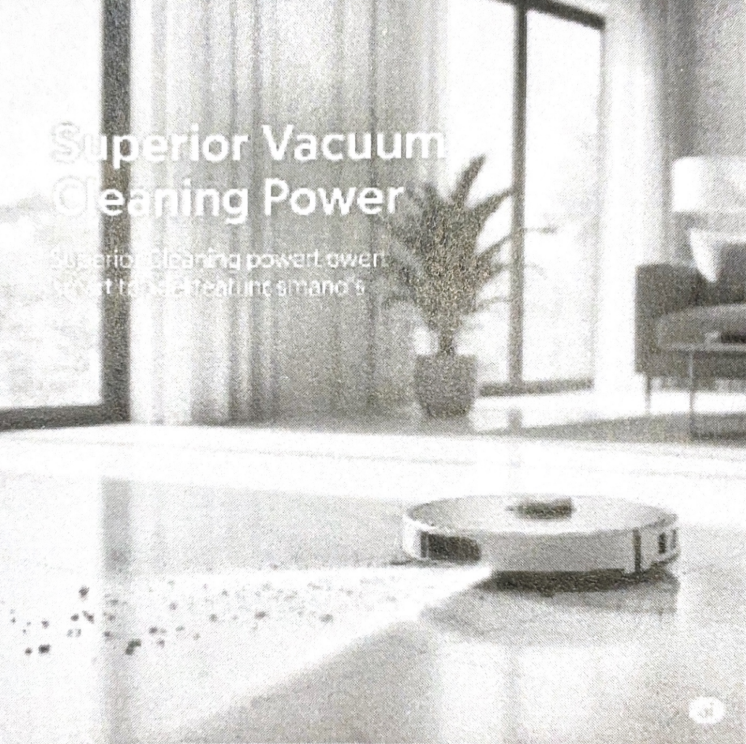
\includegraphics[width = \linewidth]{image/EngCom1.png}
\end{wrapstuff}
\colorbox{gray}{Mark ★☆☆☆☆ (terrible) Worst. Assembly. Ever.}\par
I bought this robot vacuum online, hoping to make my life easier. 
The box arrived in record time, which was a nice surprise. 
However, when I opened it, the instructions looked like they were written by a mischievous gnome who'd never seen a vacuum cleaner before! 
There were 50 tiny screws and 100 confusing diagrams. 
It said "easy assembly in 15 minutes," but after two hours, my living room looked like a robot explosion, and I was covered in sweat and tiny metal bits. 
The vacuum itself is probably great, but I'll never know because I gave up. 
I should have paid for professional assembly!
\colorbox{gray}{Sarah ★★★★☆ (good) Finally, a clean floor!}\par
I ordered this robot vacuum after seeing it advertised everywhere. 
It arrived a bit later than I expected, almost a week, but once I got it charged, it really started working its magic. 
My cat is terrified of it, which is pretty funny to watch, but my floors are spotless! 
It even goes under the sofa. 
I'm so happy I bought it, even if the delivery was a little slow.\par
\medskip
assembly (名詞) 組み立て in record time 記録的な速さで instructions (名詞) 指示，説明書\par
mischievous (形容詞) いたずらな gnome (名詞) ノーム(小人) diagrams (名詞) 図，図表\par
explosion (名詞) 爆発 terrified (形容詞) おそれた spotless (形容詞) 汚れのない，清潔な
\end{screen}
(1) What is Mark complaining about?\\
(2) What did the reviewers buy?\\
(3) What should Mark have done?\\
次の問題(4)-(8)について，英文が本文の内容と合致していたらT，していなければFと答えなさい．\\
(4) Mark was not able to assemble the robot vacuum in 15 minutes.\\
(5) Sarah received her robot vacuum in record time.\\
(6) Mark's cat was terrified of the robot vacuum. \\
(7) The robot vacuum can go under the sofa.\\
(8) Mark was satisfied with the performance of the robot vacuum.\\